                                           
\iffalse
    \title{Assignment}
    \author{EE24BTECH11028}
    \section{ee}
    \chapter{2016}
  \fi
    \item The man wno is now municipal commissioner worked as\\
    \begin{enumerate}
        \item the security guard at a university\\
        \item a security guard at a university\\
         \item a security guard at  university\\
          \item the security guard at the university   
    \end{enumerate}
    \item  Noboby knows how the indian cricket team is going to cope with the difficult and seamer-friendly wickets in Australia.\\
    
    Choose the option which is closet in meaning to the underlined phrase in the above sentance\\
    \begin{enumerate}
        \item put up with\\
        \item put in with\\
        \item put down to\\
        \item put up against
    \end{enumerate}
    \item Find the odd in the following group of words.\\
                     mock, deride, praise, jeer\\
    \begin{enumerate}
        \item mock\\
        \item deride\\
        \item praise\\
        \item jeer
    \end{enumerate}
    \item Pick the odd one from the following options.\\
    \begin{enumerate}
    \item CADBE\\
    \item JHKIL\\
    \item XVYWZ\\
    \item ONPMQ
    \end{enumerate}
    \item In a quaadratic function, the value of the product of the roots $\vec(\alpha,\beta)$ is $4$.Find the value of\\
                              $\frac{\alpha^{n} + \beta^{n}}{\alpha^{-n} + \beta^{-n}}$\\
    \begin{enumerate}
        \item$n^{4}$\\
        \item$4^{n}$\\
        \item$2^{2n-1}$\\
        \item$4^{n-1}$
        \end{enumerate}
    \item Among  faculty members in an institution,$55$ are connected with each other through facebook and $85$ are connected through WhatsApp. $30$ facult members do not have Facebook or WhatsApp accounts.The number of faculty members connected only through Facebook accounts is\\
    \begin{enumerate}
        \item$35$\\
        \item$45$\\
        \item$65$\\
        \item$90$
    \end{enumerate}
    \item Computers were invented for performing only high-end useful computations.However,it is no understatement that they taken over our world today.The internet for example ,is ubiquitous.Many believe that the internet itself is an unintended conseqquene of the original invention.With the advent of mobile computing on our phoses, a whole new dimension is enabled.One is wondering if all these development are good or, more importantly,requied.\\
    which of the statement$\brak{s}$ below is/are logically valid and be inferred from the above paragraph?\\
    $\brak{i}$ The author believes that computers are not good for us.
    $\brak{ii}$ Mobile computers and the internet are both intended inventions\\
    \begin{enumerate}
        \item $\brak{i}$ only\\
        \item $\brak{ii}$ only\\
        \item both$\brak{i}\brak{ii}$\\
        \item neither$\brak{i}\brak{ii}$
    \end{enumerate}
    \item All hill-stations a lake.Ooty has two lakes.\\
    Which of the statement$\brak{t}$ below is/are logically valid and can be inferred from the above sentances\\
    $\brak{i}$ Ooty is not ahill-station.\\
    $\brak{ii}$ No hill-station can have more than one lake.
    \begin{enumerate}
        \item $\brak{i}$ only\\
        \item$\brak{ii}$ only\\
        \item both$\brak{i}$ and $\brak{ii}$\\
        \item neither$\brak{i}$ nor $\brak{ii}$
    \end{enumerate}
    \item In a $2 * 4$ rectangle grid shown below,each cell is a rectangle.How many rectangle can be observed in the grid?\\   
    
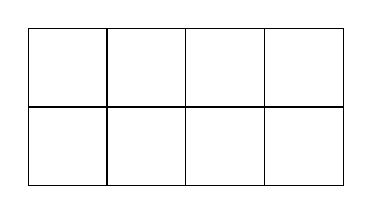
\begin{tikzpicture}
  \draw (0,0) grid (4,2);
\end{tikzpicture}
 \begin{enumerate}
    \item$21$\\
    \item$27$\\
    \item$30$\\
    \item$36$
    \end{enumerate}
    \item Choose the correct expression for $f\brak{x}$ given in the graph.
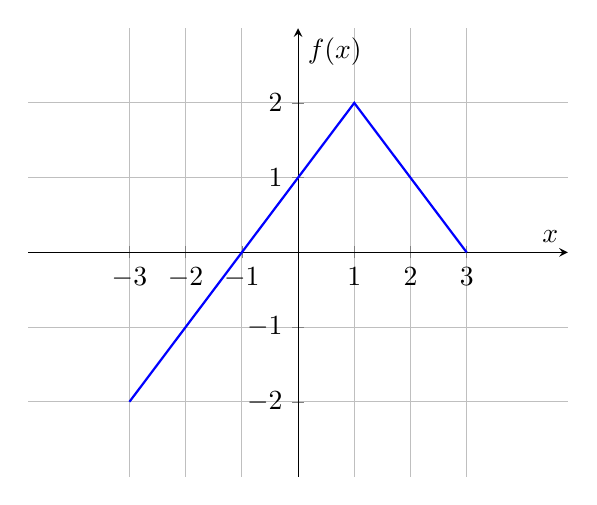
\begin{tikzpicture}
  \begin{axis}[
      axis lines=middle,
      xlabel={$x$},
      ylabel={$f(x)$},
      xmin=-4, xmax=4,
      ymin=-2.5, ymax=2.5,
      xtick={-3,-2,-1,0,1,2,3},
      ytick={-2,-1,0,1,2},
      grid=both,
      enlargelimits=true,
    ]
    % Plot the piecewise linear function
    \addplot[
      thick,
      blue,
      domain=-1:3
    ] coordinates {
       (-3,-2) (-1,0) (0,1) (1,2)  (3,0) 
    };
  \end{axis}
\end{tikzpicture}
    \begin{enumerate}
        \item $f\brak{x}=1-\abs{x-1}$\\
        \item $f\brak{x}=1+\abs{x-1}$\\
        \item $f\brak{x}=2-\abs{x-1}$\\
        \item $f\brak{x}=2+\abs{x-1}$
    \end{enumerate}
    \item The maximum value attained by the function $f\brak{x}=x\brak{x-1}\brak{x-2}$ in the interval $\sbrak{1,2}$ is.\\
    \item consider a $3 * 3$ matrix with every element being equal to 1.Its only non zero eigenvalue is.
    \item The Laplace Transform of $f\brak{t}=e^{2t}\sin\brak{5t}u\brak{t}$ is.
    \begin{enumerate}
        \item$\frac{5}{s^{2}-4s+29}$\\
        \item$\frac{5}{s^{2}+5}$\\
        \item$\frac{s-2}{s^{2}-4s+29}$\\
        \item$\frac{5}{s+5}$
    \end{enumerate}

    

